\RequirePackage[l2tabu, orthodox]{nag}
\documentclass{article}

\usepackage[letterpaper]{geometry}
\usepackage{booktabs}
\usepackage[final]{pdfpages}
\usepackage{siunitx}
\usepackage{subcaption}
\usepackage{float}

\title{CMPUT 382 Lab 4}
\author{Michael Kwok}
\begin{document}

\maketitle

The tiled matrix multiplication implementation was found to be around \( 2.54 \times \) faster than the naive matrix multiplication method, with the numbers being from \SI{82846.336}{\micro\second} to \SI{32556.640}{\micro\second}. The occupancy stayed the same at the same blocksize.


\begin{figure}[H]
    \centering
    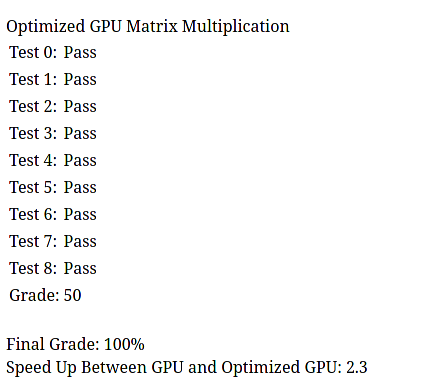
\includegraphics[width=0.6\textwidth]{grading.png}
    \caption{Automated grading result}
\end{figure}

\begin{figure}
    \centering
    \begin{subfigure}[b]{\textwidth}
        \centering
        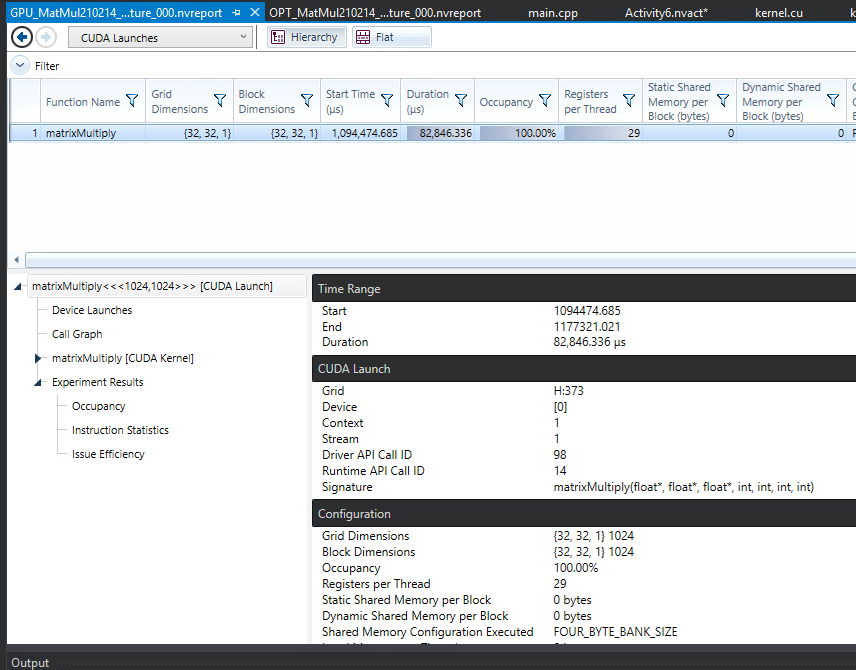
\includegraphics[width=\textwidth]{slow.png}
        \caption{Screenshot of unoptimized kernel}
    \end{subfigure}

    \begin{subfigure}[b]{\textwidth}
        \centering
        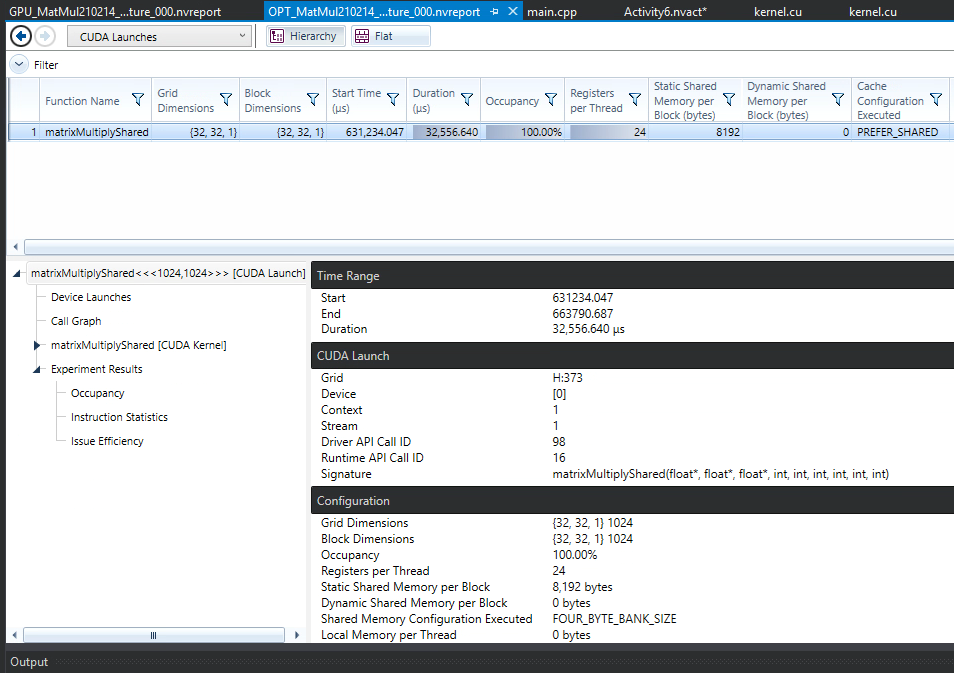
\includegraphics[width=\textwidth]{fast.png}
        \caption{Screenshot of optimized kernel}
    \end{subfigure}
    \caption{NSight Launch results}
\end{figure}

\end{document}
